\documentclass{officialexam} 
\usepackage{circuitikz}
\everymath{\color{blue}}
\usepackage{multirow}
\usepackage{chemfig}
\usepackage{tikz}
\usepackage{array}
\usepackage{circuitikz}
\usepackage{graphicx}
\graphicspath{ {./images/} }
\usepackage[version=4]{mhchem}
\begin{document}
	\maketitle\\
	\borderline{ប្រធានទី០១}
	\begin{enumerate}[I]
		\item {\color{khtug}\sffamily ចូរគូសសញ្ញា $\left(\tick \right)$ ក្នុងប្រអប់ខាងមុខចម្លើយត្រឹមត្រូវៈ}
		\begin{enumerate}[m]
			\item បំបែកកម្លាំងមួយជាកម្លាំងផ្គុំពីរ គឺំនួសកម្លាំងនោះដោយកម្លាំងពីរដែលផ្តល់ៈ
			\begin{multicols}{2}
				\begin{enumerate}[bk]
					\item ផលដូចកម្លាំងដើម
					\item ផលផ្ទុយកម្លាំងដើម
					\item ផលស្របកម្លាំងដើម
					\item ផលច្រាសកម្លាំងដើម
				\end{enumerate}
			\end{multicols}
		\item ទំហំកំណត់ដោយផលគុណរវាងកម្លាំង និងប្រវែងដៃឃ្នាស់ហៅថាៈ
		\begin{multicols}{2}
			\begin{enumerate}[bk]
				\item ម៉ូម៉ង់នៃឃ្នាស់
				\item ម៉ូម៉ង់នៃកម្លាំង
				\item ម៉ូម៉ង់ប្លង់ទេរ
				\item ម៉ូម៉ង់កង់យោង
			\end{enumerate}
		\end{multicols}
		\end{enumerate}
		\item {\color{khtug}\sffamily ចូរបំពេញល្បះខាងក្រោមឲ្យបានត្រឹមត្រូវៈ}
		\begin{enumerate}[m]
			\item ម៉ូម៉ង់កម្លាំងដែលធ្វើឲ្យអង្គធាតុវិលតាមទិសដៅទ្រនិចនាឡិកាជា\dotfill ។
			\item ម៉ូម៉ង់កម្លាំងដែលធ្វើឲ្យអង្គធាតុវិលតាមទិសដៅច្រាសទ្រនិចនាឡិកាជា\dotfill ។
			\item បង្គុំកម្លាំងពីរស្របគ្នាជាកម្លាំង\dotfill។
			\item បានជាគេយកដៃរុញទ្វារក្បែរត្រចៀកវាពិបាកបើក ព្រោះខ្សែសកម្មនៃកម្លាំងស្ថិតនៅជិតអ័ក្សរង្វិល ដូចនេះយើងត្រូវបញ្ចេញកម្លាំង\dotfill។
		\end{enumerate} 
		\item {\color{khtug}\sffamily ចូរផ្គូផ្គងផ្នែក $\left(A\right)$ និង $\left(B\right)$ ឲ្យបានត្រឹមត្រូវ}\\
		\begin{center}
			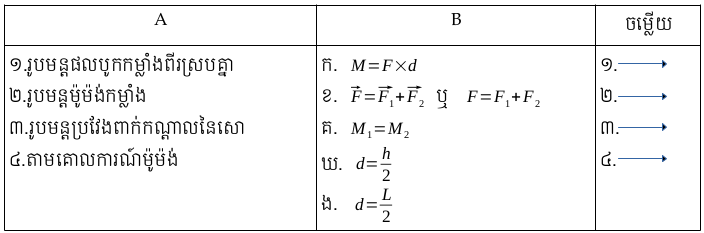
\includegraphics[scale=0.6]{17}
		\end{center}
		\item {\color{khtug}\sffamily លំហាត់}
		\begin{enumerate}[m]
			\item បន្ទាត់ស្មើសាច់មួយមានប្រវែង $50cm$ ចុងទាំងសងខាងនៃបន្ទាត់រងនូវកម្លាំងពីរស្របគ្នា និងមានទិសដៅដូចគ្នា។ កម្លាំងទីមួយស្មើនឹង $800N$ កម្លាំងទីពីរស្មើនឹង $600N$។ កំណត់កម្លាំងផ្គួបទាំងពីរ។
			\item គេមានកម្លាំងពីរ $\overrightarrow{F}_1$ និង $\overrightarrow{F}_2$ កែងគ្នាមានអាំងតង់សុីតេរៀងគ្នា $4N$ និង $8N$ ហើយមានចំណុចចាប់រួម $O$។
			\begin{enumerate}[k]
				\item គូសវុិចទ័រតាងកម្លាំងផ្គួបនៃកម្លាំងទាំងពីរ។
				\item រកអាំងតង់សុីតេកម្លាំងផ្គួបដោយប្រើមាត្រដ្ឋាន $1cm=1N$។
			\end{enumerate}
			\item ក្នេងប្រុសម្នាក់មានទម្ងន់ $400N$ អង្គុយនៅលើចុងម្ខាងនៃដង់ថ្លឹងចម្ងាយ $1.2m$ ពីអ័ក្សរង្វិល។ ដើម្បីឲ្យដងថ្លឹងមានលំនឹងតាមទិសដេក គេដាក់ក្មេងប្រុសម្នាក់ទៀត ឲ្យអង្គុយនៅចុងម្ខាងនៃដងថ្លឹងដែលមានប្រវែង $2.6m$ ពីអ័ក្សរង្វិល។ តើគេត្រូវដាក់ក្មេងប្រុសម្នាក់ទៀតមានទម្ងន់ប៉ុន្មានញ៉ូតុន $\left(N\right)$?
		\end{enumerate}
	\end{enumerate}
\borderline{ដំណោះស្រាយ}\\
{\color{white}.}\dotfill
\\
{\color{white}.}\dotfill\\
{\color{white}.}\dotfill\\
{\color{white}.}\dotfill
\\
{\color{white}.}\dotfill\\
{\color{white}.}\dotfill\\
{\color{white}.}\dotfill
\\
{\color{white}.}\dotfill\\
{\color{white}.}\dotfill\\
{\color{white}.}\dotfill
\\
{\color{white}.}\dotfill\\
{\color{white}.}\dotfill\\
{\color{white}.}\dotfill
\\
{\color{white}.}\dotfill\\
{\color{white}.}\dotfill\\
{\color{white}.}\dotfill
\\
{\color{white}.}\dotfill\\
{\color{white}.}\dotfill\\
{\color{white}.}\dotfill
\\
{\color{white}.}\dotfill\\
{\color{white}.}\dotfill
\begin{center}
	\sffamily\color{blue}
	សូមសំណាងល្អ!
\end{center}\newpage
\maketitle\\
\borderline{ប្រធានទី០២}
\begin{enumerate}[I]
	\item {\color{khtug}\sffamily ចូរគូសសញ្ញា $\left(\tick\right)$ }
\end{enumerate}
\borderline{ដំណោះស្រាយ}\\
{\color{white}.}\dotfill
\\
{\color{white}.}\dotfill\\
{\color{white}.}\dotfill\\
{\color{white}.}\dotfill
\\
{\color{white}.}\dotfill\\
{\color{white}.}\dotfill\\
{\color{white}.}\dotfill
\\
{\color{white}.}\dotfill\\
{\color{white}.}\dotfill\\
{\color{white}.}\dotfill
\\
{\color{white}.}\dotfill\\
{\color{white}.}\dotfill\\
{\color{white}.}\dotfill
\\
{\color{white}.}\dotfill\\
{\color{white}.}\dotfill\\
{\color{white}.}\dotfill
\\
{\color{white}.}\dotfill\\
{\color{white}.}\dotfill\\
{\color{white}.}\dotfill
\\
{\color{white}.}\dotfill\\
{\color{white}.}\dotfill
\begin{center}
	\sffamily\color{blue}
	សូមសំណាងល្អ!
\end{center}\newpage
\end{document}